\section{Performance measurement}\label{Performance Measurement}


We will now discuss the feasibility of the proposed load balancer by comparing 
its performance with those of existing iptables DNAT and the Nginx based load balancers. 
We conducted the performance measurements using the benchmark program called wrk\cite{Glozer2016}.

We also investigated the performance varying two network configurations: 
First one is an overlay network setting\cite{Sill2016,Marmol2015} that is often used to build the Kubernetes cluster. 
Flannel\cite{CoreOSFlannel} is one of popular overlay network technologies. 
We compared the performances of three backends settings\cite{CoreOSFlannelBackend}, 
{\it i.e.} operating modes of flannel, to find the best setting.
The other one is the setting for distributed packet processing.
It is well known that distributing handling of interrupts from the network interface card(NIC) 
and the subsequent IP protocol processing, among multiple cores impact the network performance.
In order to derive the best performance from load balancers, 
we also investigated how this setting would affect their performance.

The following subsections explain these in further detail. 

\subsection{Benchmark method}

\begin{figure}
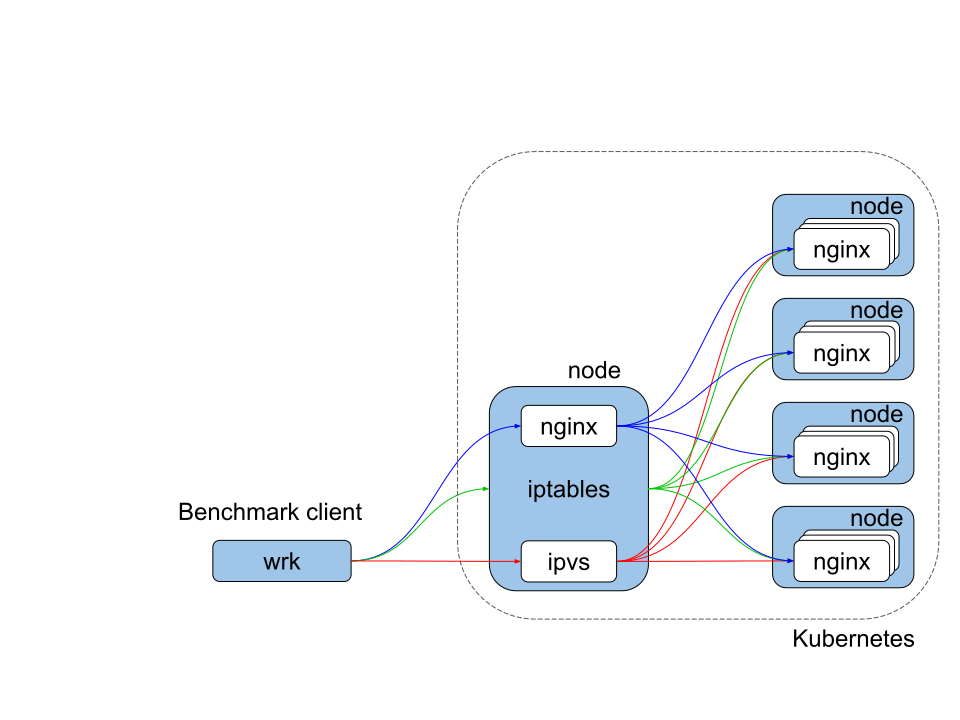
\includegraphics[width=\columnwidth]{Figs/benchmark-schem}
\caption{Benchmark setup}
\label{fig:benchmark-schem}
\end{figure}

We measured the performance of the load balancers using the wrk.
Figure~\ref{fig:benchmark-schem} illustrates a schematic diagram of our experimental setup.
Multiple {\em pods} are deployed on multiple nodes in the Kubernetes cluster. 
In each {\em pod}, a Nginx web server that returns the IP address of the {\em pod} are running.
We then set up the IPVS, iptables DNAT, and Nginx load balancers on one of the nodes(the top right node in the Figure~\ref{fig:benchmark-schem}). 

We measured the throughput, Request/sec, of the web service running on the Kubernetes cluster as follows:
The HTTP GET requests are sent out by the wrk on the client machine toward the nodes,
using destination IP addresses and port numbers that are chosen based on the type of the load balancer on which the measurement is performed.
The load balancer on the node then distributes the requests to the {\em pods}.
Each {\em pod} will return HTTP responses to the load balancer, after which the load balancer returns them to the client.
Based on the number of responses received by wrk on the client, 
load balancer performance, in terms of Request/sec can be obtained. 

Figure~\ref{fig:benchmark example} shows an example of the command-line for wrk and the corresponding output.
The command-line in Figure~\ref{fig:benchmark example} will generate 40 wrk program threads 
and allow those threads to send out a total of 800 concurrent HTTP requests over the period of 30 seconds.
The output example shows information including per thread statistics, error counts, Request/sec and Transfer/sec.

Figure~\ref{fig:Hardware and software configuration} shows hardware and software configuration used in our experiments.
We configured Nginx HTTP server to return a small HTTP content, 
the IP address of the {\em pod}, to make a relatively severe condition for load balancers. 
The size of the character string making up an IP address is limited to 15 bytes.
If we had chosen the HTTP response size so that most of the IP packet resulted in maximum transmission unit(MTU), 
the performance would have been limited by the Ethernet bandwidth.
However, since we used small HTTP responses, we could purely measure the load balancer performance.

The hardware we used had eight physical CPU cores and a NIC with 4 rx-queues.

\begin{figure}
\begin{minipage}{\columnwidth}
\small
\begin{Verbatim}[commandchars=\\\{\}]
\underline{\textbf{Command line:}}
 wrk -c800 -t40 -d30s http://172.16.72.2:8888/
-c: concurrency, -t: # of thread, -d: duration

\underline{\textbf{Output example:}}
 Running 30s test @ http://10.254.0.10:81/
  40 threads and 800 connections
  Thread Stats   Avg      Stdev     Max   +/- Stdev
    Latency    15.82ms   41.45ms   1.90s    91.90%
    Req/Sec     4.14k   342.26     6.45k    69.24%
  4958000 requests in 30.10s, 1.14GB read
  Socket errors: connect 0, read 0, write 0, timeout 1
Requests/sec: 164717.63
Transfer/sec:     38.86MB
\end{Verbatim}
\end{minipage}
\caption{Example output of benchmark by wrk}
\label{fig:benchmark example}
\end{figure}

\begin{figure}
\begin{minipage}{0.9\columnwidth}
\small
\begin{Verbatim}[commandchars=\\\{\}]
\underline{\textbf{Physical Machine Specification:}}
  CPU: Intel(R) Xeon(R) CPU E5-2450 0 @ 2.10GHz
  # of Physical Cores: 8
  Hyper Threading: enabled
  Memory: 32GB
  NIC: Broadcom BCM5720 Gigabit Ethernet PCIe

\underline{\textbf{Number of Physical Machines:}}
  Master: 1
  Node: 7
  Client: 1

\underline{\textbf{Node Software version:}}
  OS: Debian 8.7 (Jessie)
  Kernel: \footnotesize{3.16.0-4-amd64 #1 SMP Debian 3.16.39-1 (2016-12-30)}
  Kubernetes v1.5.2
  flannel v0.7.0
  etcd version: 3.0.15

\underline{\textbf{Load balancer Software version:}}
  Keepalived: v1.3.2 (12/03,2016)
  Nginx: nginx/1.11.1

\underline{\textbf{Worker Pod Software version:}}
  nginx : nginx/1.13.0 
\end{Verbatim}
\end{minipage}
\caption{Hardware and software configuration}
\label{fig:Hardware and software configuration}
\end{figure}


\subsection{Overlay network}

We used flannel to build the Kubernetes cluster used in our experiment.
Flannel has three types of backend, {\it i.e.}, operating modes, named host-gw, vxlan, and udp\cite{CoreOSFlannelBackend}.

In the host-gw mode, the flanneld installed on a node simply configures the routing table 
based on the IP address assignment information of the overlay network, which is stored in the etcd. 
When a {\em pod} on a node sends out an IP packet to {\em pods} on the different node, 
the former node consults the routing table and learn that the IP packet should be sent out to the latter.
Then, the former node forms Ethernet frames containing the destination MAC address of the latter node 
without changing the IP header, and send them out.

In the case of the vxlan mode, flanneld creates the Linux kernel's vxlan device, flannel.1. 
Flanneld will also configures the routing table appropriately based on the information stored in the etcd.
When {\em pods} on different nodes need to communicate, the packet is routed to flannel.1.
The vxlan functionality of the Linux kernel identify the MAC address of flannel.1 device on the destination node,
then form an Ethernet frame toward the MAC address.
The vxlan then encapsulates the Ethernet frame in a UDP/IP packet with a vxlan header, after which the IP packet is eventually sent out.

In the case of udp mode, flanneld creates the tun device, flannel0, and configures the routing table.
The flannel0 device is connected to the flanneld daemon itself.
An IP packet routed to flannel0 is encapsulated by flanneld, and eventually sent out 
to the appropriate node. 
The encapsulation is done for IP packets.

Figure~\ref{fig:flannel-packet-diagram} shows the schematic diagrams of frame formats for three backends modes of the flannel overlay network. 
The MTU sizes in the backends, assuming the MTU size without encapsulation is 1500 bytes, are also presented.
Since packets are not encapsulated in the host-gw mode, the MTU size remains 1500 bytes.
An additional 50 bytes of header is used in the vxlan mode, thereby resulting in an MTU size of 1450 bytes.
In the case of the udp mode, only 28 bytes of header are used for encapsulation, which results in an MTU size of 1472 bytes.

\begin{figure}
\includegraphics[width=\columnwidth]{Figs/flannel-packet-diagram}
\caption{frame diagram}
\label{fig:flannel-packet-diagram}
\end{figure}

Performance of the load balancers can be influenced by the overhead of encapsulation. 
Thus, the host-gw mode, where there is no overhead due to encapsulation, 
results in the best performance levels as shown in Section~\ref{Result and Discussion}.
However, the host-gw mode has a significant drawback that prohibit it to work correctly in cloud platforms. 
Since the host-gw mode simply sends out a packet without encapsulation, if there is a cloud gateway between nodes, 
the gateway cannot identify the proper destination, thus drop the packet.

\begin{table}
  \begin{tabular}{lccc}
    \toprule
    flannel backend & On-premise & GCP & AWS \\
    \midrule
    host-gw & OK & NG & (OK) \\
    vxlan & OK & OK & OK \\
    udp & OK & OK & OK \\
    \bottomrule
\end{tabular}

  \caption{Viable flannel backend modes}
  \label{tab:Viable flannel backends}
\end{table}

We conducted an investigation to determine which of the flannel backend mode would be usable on AWS, GCP, and on-premise data centers.
The results are summarized in Table~\ref{tab:Viable flannel backends}. 
In the case of GCP, an IP address of {\tt /32} is assigned to every VM host and 
every communication between VMs goes through GCP's gateway.
As for AWS, the VMs within the same subnet communicate directly, while the VMs in different subnets communicate via the AWS's gateway.
Since the  gateways do not have knowledge of the flannel overlay network, they drop the packets; thereby, 
they prohibit the use of the flannel host-gw mode in those cloud providers.  

In our experiment, we compared the performance of load balancers when different flannel backend modes were used. 

\subsection{Distributed packet handling}

Recently, the performance of CPUs are improved significantly due to the development of multi-core CPUs.
One of the top of the line server processors from Intel now includes up to 28 cores in a single CPU.
In order to enjoy the benefits of multi-core CPUs in communication performance, 
it is necessary to distribute the handling of interrupts from the NIC and the IP protocol processing
to the available physical cores.
Receive Side Scaling (RSS)\cite{TomHerbert} is a technology 
to distribute handling of the interrupt from NIC queues to multiple CPU cores.
Subsequently, Receive Packet Steering (RPS)\cite{TomHerbert} distributes the IP protocol processing 
to multiple CPU cores by issuing inter core software interrupts.

Since load balancer performance levels could be affected by these technologies,
we conducted an experiment to determine how load balancer performance level change depending on the RSS and RPS settings.
The following shows how RSS and RPS are enabled and disabled in our experiment. 
The NIC used in our experiment is Broadcom BCM5720, which has four rx-queues and one tx-queue.
Figure~\ref{fig:rx-queue} shows the interrupt request (IRQ) number assignments to those NIC queues.

\begin{figure}
%\begin{center}
\begin{minipage}{0.7\columnwidth}
\small
\begin{verbatim}
81: eth0-tx-0
82: eth0-rx-1
83: eth0-rx-2
84: eth0-rx-3
85: eth0-rx-4
# obtained from /proc/interrupts 
\end{verbatim}
\end{minipage}
\caption{RX/TX queues of the hardware}
\label{fig:rx-queue}
%\end{center}
\end{figure}

When packets arrive, they are distributed to these rx-queues depending on the flow each packet belongs to.
Each receive queue has a separate IRQ associated with it. The NIC triggers
this to notify a CPU when new packets arrive on the given queue.
Then, the notified CPU handles the interrupt, and performs the protocol processing. 
According to the \cite{TomHerbert}, the CPU cores allowed to be notified is controlled by setting 
a hexadecimal value corresponding to the bit maps indicating the allowed CPU cores in \enquote{/proc/irq/\$irq\_number /smp\_affinity}.
%
For example, in order to route the interrupt for eth0-rx-1 to CPU0, 
we should set \enquote{/proc/irq/82/smp\_affinity} 
to binary number {\tt 0001}, which is 1 in hexadecimal value.
Further, in order to route the interrupt for eth0-rx-2 to CPU1, we 
should set \enquote{/proc/irq/83/smp\_affinity} 
to binary number {\tt 0010}, which is 2 in hexadecimal value.

We refer the setting to distribute interrupts from four rx-queues to CPU0, CPU1, CPU2 and CPU3 as {\tt RSS = on}. 
It is configured as the following setting: 

\begin{center}
\begin{minipage}{0.8\columnwidth}
\begin{Verbatim}[commandchars=\\\{\}]

\underline{\textbf{RSS=on}}
echo 1 > /proc/irq/82/smp_affinity
echo 2 > /proc/irq/83/smp_affinity
echo 4 > /proc/irq/84/smp_affinity
echo 8 > /proc/irq/85/smp_affinity

\end{Verbatim}
\end{minipage}
\end{center}

On the other hand, {\tt RSS = off} means that an interrupt from any rx-queue is routed to CPU0. 
It is configured as the following setting:

\begin{center}
\begin{minipage}{0.8\columnwidth}
\begin{Verbatim}[commandchars=\\\{\}]

\underline{\textbf{RSS=off}}
echo 1 > /proc/irq/82/smp_affinity
echo 1 > /proc/irq/83/smp_affinity
echo 1 > /proc/irq/84/smp_affinity
echo 1 > /proc/irq/85/smp_affinity

\end{Verbatim}
\end{minipage}
\end{center}

%In this case, interrupt from any of rx-queue is routed to CPU0.

The RPS distributes IP protocol processing by placing the packet
on the desired CPU's backlog queue and wakes up the CPU using inter-processor interrupts.
We have used the following settings to enable the RPS:

\begin{center}
\begin{minipage}{0.95\columnwidth}
\begin{Verbatim}[commandchars=\\\{\}]

\underline{\textbf{RPS=on}}
echo fefe > /sys/class/net/eth0/queues/rx-0/RPS_cpus
echo fefe > /sys/class/net/eth0/queues/rx-1/RPS_cpus
echo fefe > /sys/class/net/eth0/queues/rx-2/RPS_cpus
echo fefe > /sys/class/net/eth0/queues/rx-3/RPS_cpus

\end{Verbatim}
\end{minipage}
\end{center}

Since the hexadecimal value \enquote{fefe} represented as \enquote{1111 1110 1111 1110} in binary, 
this setting will allow distributing protocol processing to all of the CPUs, except for CPU0 and CPU8.
In this paper, we will refer this setting as {\tt RPS = on}.
%
On the other hand, {\tt RPS = off} means that no CPU is allowed for RPS. 
Here, the IP protocol processing is performed on the CPUs the initial hardware interrupt is received.
It is configured as the following settings:

\begin{center}
\begin{minipage}{0.9\columnwidth}
\begin{Verbatim}[commandchars=\\\{\}]

\underline{\textbf{RPS=off}}
echo 0 > /sys/class/net/eth0/queues/rx-0/RPS_cpus
echo 0 > /sys/class/net/eth0/queues/rx-1/RPS_cpus
echo 0 > /sys/class/net/eth0/queues/rx-2/RPS_cpus
echo 0 > /sys/class/net/eth0/queues/rx-3/RPS_cpus

\end{Verbatim}
\end{minipage}
\end{center}

The RPS is especially effective when the NIC does not have multiple receive queues or when the number of queues is 
much smaller than the number of CPU cores. 
That was the case of our experiment, where we had a NIC with only four rx-queues, 
while there was a CPU with eight physical cores.

\section{Result and Discussion}\label{Result and Discussion}

\begin{figure}
\includegraphics[width=0.6\columnwidth]{Figs/ipvs_3figs}
\caption{IPVS results}
\label{fig:IPVS3figs}
\end{figure}

\begin{figure}
\includegraphics[width=\columnwidth]{Figs/performance_limitation}
\caption{Performance limitation due to 1Gbps bandwidth}
\label{fig:performance_limitation}
\end{figure}

\begin{figure}
\includegraphics[width=0.6\columnwidth]{Figs/iptables_3figs}
\caption{iptables results}
\label{fig:iptabls3figs}
\end{figure}

\begin{figure}
\includegraphics[width=\columnwidth]{Figs/ipvs-iptables-nginx_2figs}
\caption{IPVS and iptables comparison}
\label{fig:IPVS-iptables-nginx_2figs}
\end{figure}

\begin{figure}
\includegraphics[width=\columnwidth]{Figs/latency_cdf_rps_40pods}
\caption{Latency cumulative distribution function}
\label{fig:latency_cdf_rps_40pods}
\end{figure}


Figure~\ref{fig:IPVS3figs} shows the IPVS load balancer performance, that is, 
the throughput (Request/sec) of the Nginx web server {\em pods} in our experiments.
As for the overlay network, we measured the performance for three flannel backend modes, 
host-gw (Figure~\ref{fig:IPVS3figs}(a)), vxlan (Figure~\ref{fig:IPVS3figs}(b)) and udp (Figure~\ref{fig:IPVS3figs}(c)).
The following RSS and RPS setting were compared: 

\begin{center}
\begin{minipage}{0.8\columnwidth}
\begin{verbatim}
(RSS, RPS) = (off, off)
           = (on , off)
           = (off, on )
\end{verbatim}
\end{minipage}
\end{center}

Except for the udp cases, we can see the trend in which the throughput linearly increases 
as the {\em pod} number increases and then it eventually saturates.
The saturated performance levels indicates the maximum performance of the IPVS load balancer.
The maximum performance limits depend on the flannel backend mode type and the (RSS, RPS) settings.
From the results in Figures~\ref{fig:IPVS3figs}(a,b), it can be seen that if we turn off distributed packet processing,
{\it i.e.}, when \enquote{(RSS, RPS) = (off, off)}, performance degrades significantly. 
In this case, the performance bottleneck is primarily due to packet processing in a single core.

If we compare the results for the cases when \enquote{(RSS, RPS) = (on, off)} and \enquote{(RSS, RPS) = (off, on)},
the latter is better than the former.
This is understandable, since in the case of \enquote{RPS = on}, eight physical cores can be used whereas 
in the case of \enquote{RSS = on} only four cores can be used, on the hardware used in our experiment.
The performance bottleneck of the case when \enquote{RSS = on} is considered 
to be due to the fact that the packet processing is only done on four CPU cores.
%
At first, it was not clear what caused the performance limit for the case when \enquote{RPS = on},
however we now suspect this is due to 1Gbps bandwidth limitation.
A packet level analysis using tcpdump\cite{jacobson1989tcpdump} revealed that 622.72 byte of extra HTTP headers, 
TCP/IP headers and ethernet frames are needed for each request in the case of the wrk benchmack program.  
This results in the upper limitation of 196,627 [req/s], where the date size of HTTP response body is 13 byte, or typical data size in our experiment. 
Figure~\ref{fig:performance_limitation} shows upper limitation of the performance level for 1Gbps ethernet together with 
actual benchmark results and we can conclude that when \enquote{RPS = on}, IPVS performance is limited by bandwidth.

If we compare the performances among the flannel backend modes types, 
the host-gw mode where no encapsulation is conducted shows the highest performance level,
followed by the vxlan mode where the Linux kernel encapsulate the Ethernet frame.
The udp mode where flanneld itself encapsulate the IP packet shows significantly lower performances levels.

Figure~\ref{fig:iptabls3figs} shows the performance of the load balancer 
functionality of the iptables DNAT. 
As can be seen in the figure, the performance value increases as the number of the {\em pod} increases linearly, 
and then becomes saturated at some point, as was the case with the IPVS results.

If we compare the results for different packet handling settings, the highest performance is 
obtained for the case when \enquote{(RSS, RPS) = (off on)}, followed by the case when \enquote{(RSS, RPS) = (on, off)}. 
The performance result for the case when \enquote{(RSS, RPS) = (off, off)} resulted in the 
poorest performance level, as was the case for the IPVS.
As for the flannel backend modes, the host-gw shows the highest performance followed 
by the vxlan. The udp backend mode totally degrades the performance level.

Figure~\ref{fig:IPVS-iptables-nginx_2figs} compares the performance measurement results 
among the IPVS, iptables DNAT, and Nginx load balancers
with the condition of \enquote{(RSS, RPS) = (off on)}.
The proposed IPVS load balancer exhibits almost equivalent performance as the existing iptables DNAT based load balancer. 
The Nginx based load balancer shows no performance improvement even though the number of the Nginx web server {\em pods} is increased.
It is understandable because the performance of the Nginx as a load balancer is expected to be similar to the performance as a web server.
Figure~\ref{fig:latency_cdf_rps_40pods} compares Cumulative Distribution Function(CDF) of the load balancer latency at the constant load.
The latencies are a little bit smaller for IPVS, however we consider the difference almost negligible.
For example, the median value at 160K[req/s] load for IPVS and iptables DNAT are, 1.1 msec and 1.2 msec, respectively.
So, we can conclude our proposed load balancer showed no performance degradation while providing potability.
